%%%%%%%%%%%%%%%%%%%%%%%%%%%%%%%%%%%%%%%%%
%%% HYPERRIDE Reporting Template
%%%%%%%%%%%%%%%%%%%%%%%%%%%%%%%%%%%%%%%%%

\documentclass[letterpaper,12pt]{report}
\usepackage[pass]{geometry}
\usepackage{hyperride}		% HYPERRIDE specific definitions and styles  
\usepackage[utf8]{inputenc}	% UTF8 package
\usepackage[T1]{fontenc}
\usepackage{textcomp}		% common special chars
\usepackage{amsmath}		% math formula
\usepackage{fancybox}
\usepackage{anyfontsize}	% fonts
\usepackage{lipsum}
\usepackage{float}
\usepackage[normalem]{ulem}
\usepackage{cleveref}
\usepackage[printonlyused]{acronym}
\hypersetup{
	pdftitle={Beacon Network Security Labs: Evil Twin Attack Detection Lab Setup},
	pdfauthor={[Jordan Whyte, Gaby Dagher]},
	pdfkeywords={Beacon Labs, Evil Twin, Attack Detection, Network Security},
}

\usepackage{subfigure}
\usepackage{graphicx}
\usepackage{xcolor}
\usepackage{soul}
\sethlcolor{lightgray}
\usepackage[export]{adjustbox}
\usepackage{mdframed}
\usepackage{pdfpages}
\usepackage{comment}
\usepackage{multirow,array}
\def\todo#1{{\color{hyperridered}\textbf{TODO:} ``#1''}}
\def\hyperride{HYPERRIDE}
\usepackage{mdframed}
\definecolor{lightblue}{rgb}{0.93, 0.95, 1.0}

\graphicspath{ {graphics/} }

%%%%%%%%%%%%%%%%%%%%%%%%%%%%%%%%%%%%%%%%%
%%% Definitions
%%%%%%%%%%%%%%%%%%%%%%%%%%%%%%%%%%%%%%%%%

\begin{document}

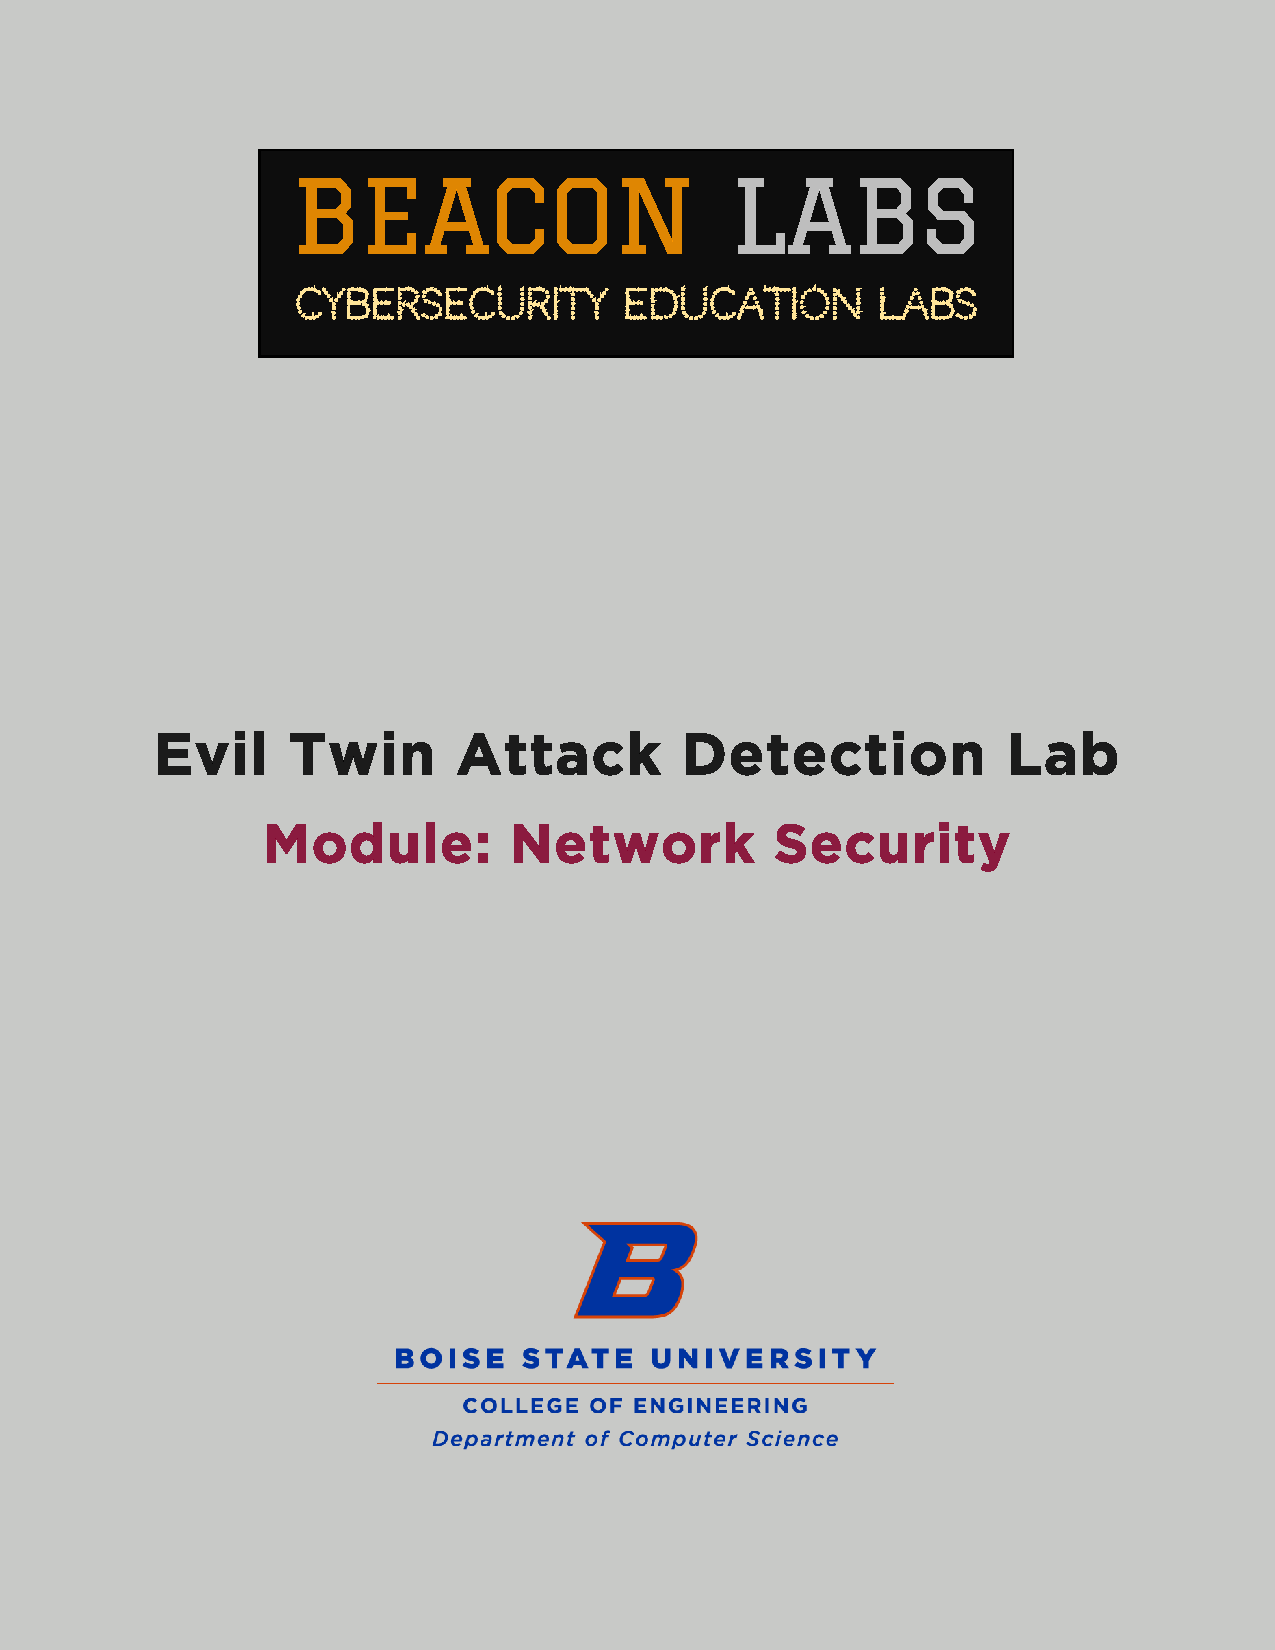
\includepdf[pages=1]{./graphics/3FP.pdf}

\mdfdefinestyle{code}{%
    linecolor=black,
    outerlinewidth=2pt,
    %roundcorner=20pt,
    innertopmargin=4pt,
    innerbottommargin=4pt,
    innerrightmargin=4pt,
    innerleftmargin=4pt,
        leftmargin = 4pt,
        rightmargin = 4pt
    backgroundcolor=black!10
    }%

\setcounter{tocdepth}{4}
\setcounter{secnumdepth}{4}

%%%%%%%%%%%%%%%%%%%%%%%%%%%%%%%%%%%%%%%%%
%%% URL style same as regular text
%%%%%%%%%%%%%%%%%%%%%%%%%%%%%%%%%%%%%%%%%
	
\urlstyle{same}

%%%%%%%%%%%%%%%%%%%%%%%%%%%%%%%%%%%%%%%%%
%%% Deliverable Information
%%%%%%%%%%%%%%%%%%%%%%%%%%%%%%%%%%%%%%%%%

% Project Meta Information
\ProjectFullTitle{Beacon Network Security Labs: Evil Scout}
\ProjectAcronym{HYPERRIDE}
\ProjectRefNo{957788}

% Report Number, use either "1", "2", or "3" for the corresponding reporting period
\delivNumber{0}

% Period covered by the report
\delivFrom{dd/mm/yyyy}
\delivTo{dd/mm/yyyy}

% Report Responsible Partner
\delivResponsible{AIT Austrian Institute of Technology (AIT)} 

% Report Version, Contractual and Actual Date, Dissemination Level, Type
\delivVersion{vn.n}
\ContractualDate{dd/mm/yyyy}
\ActualDate{dd/mm/yyyy}

% List of Main Authors (usually from the responsible partner)
\delivAuthor{[Jordan Whyte, Gaby Dagher]}

% List of Co-Authors (all other co-authors should be listed here)
\delivFPAuthor{[]}

% Report Status
\delivStatus{d} %% d = draft, f = final, s = submitted

%%%%%%%%%%%%%%%%%%%%%%%%%%%%%%%%%%%%%%%%%
%%% Change Log
%%%%%%%%%%%%%%%%%%%%%%%%%%%%%%%%%%%%%%%%%

\istChange{dd/mm/yyyy}{v1.0}{Name (Partner short name)}{Draft report template}
\istChange{}{}{}{}

%%%%%%%%%%%%%%%%%%%%%%%%%%%%%%%%%%%%%%%%%
%%% Cover Page
%%%%%%%%%%%%%%%%%%%%%%%%%%%%%%%%%%%%%%%%%

%\makecover

%%%%%%%%%%%%%%%%%%%%%%%%%%%%%%%%%%%%%%%%%
%%% Table of Contents
%%%%%%%%%%%%%%%%%%%%%%%%%%%%%%%%%%%%%%%%%

\clearpage
\fancypagestyle{plain}{}
\settableofcontents
\tableofcontents
\clearpage

%%%%%%%%%%%%%%%%%%%%%%%%%%%%%%%%%%%%%%%%%
%%% Overview
%%%%%%%%%%%%%%%%%%%%%%%%%%%%%%%%%%%%%%%%%
\newpage
\section*{Overview}\label{sec:work-carried-out}
\addcontentsline{toc}{section}{Overview}

\textbf{Objective}

Develop a comprehensive understanding of the intricacies involved in executing an Evil Twin attack, as well as devising defensive strategies from the perspective of the legitimate access point (LAP).

\textbf{Evil Twin Attacks}

Evil Twin attacks refer to a class of cybersecurity attacks where an attacker creates a rogue WiFi network that mimics a legitimate one. These types of attacks are typically executed on public WiFi networks, which are prone to many threats due to their open nature. By replicating the name and MAC address of a legitimate WiFi network, the attacker deceives clients into connecting to their network instead. This allows the attacker to perform a man-in-the-middle attack, intercepting and potentially altering the client's communication.

Previously, the only defense against this was for clients to modify their devices or for the network admin(s) to take additional measures to prevent it. However, Shrivastava et al.$^\text{[\citeauthor{Shrivastava:2020}]}$ proposed a simple and lightweight piece of code known as Evil Scout to prevent Evil Twin attacks on open WiFi networks.

In this lab, you will use a program called Mininet-WiFi which allows for the simulation of a WiFi topology to perform this attack on.

\textbf{Resources}

\textit{Paper that the attack and defense are based upon:}

P. Shrivastava, M. S. Jamal and K. Kataoka, "EvilScout: Detection and mitigation of evil twin attack in SDN enabled WiFi", IEEE Transactions on Network and Service Management, vol. 17, no. 1, pp. 89-102, 2020.$^\text{[\citeauthor{Shrivastava:2020}]}$

%%%%%%%%%%%%%%%%%%%%%%%%%%%%%%%%%%%%%%%%%
%%% Virtual Machine Setup
%%%%%%%%%%%%%%%%%%%%%%%%%%%%%%%%%%%%%%%%%

\section*{Virtual Machine Setup}\label{sec:Virtual-Machine-Setup}
\addcontentsline{toc}{section}{Virtual Machine Setup}

A premade virtual machine image will be used. It requires at least 15 GB of space, and it is recommended to allocate a minimum of 2 GB of RAM. The virtual machine contains all the files necessary to run this lab.

By understanding how this attack is executed and how to prevent it, you will gain a deeper understanding of the security vulnerabilities of public WiFi and the importance of secure network practices.

For setup instructions, see the provided Setup document.

%%%%%%%%%%%%%%%%%%%%%%%%%%%%%%%%%%%%%%%%%%%%%%%%%%%%%%%%%%%%%
%%% Lab Task Set 1: Creating the Network with Mininet-wifi
%%%%%%%%%%%%%%%%%%%%%%%%%%%%%%%%%%%%%%%%%%%%%%%%%%%%%%%%%%%%%

\section*{Task Set 1: Creating the Network with Mininet-WiFi}\label{sec:Task-Set-1}
\addcontentsline{toc}{section}{Task Set 1: Creating the Network with Mininet-WiFi}

\textbf{Objective}

Simulate the network topology in which an Evil Twin attack will be performed in order to enhance comprehension of the attack dynamics and how it can be defended against.

\subsection*{Task 1.1: Simulating the Network Topology}\label{sec:Task-1.1-Simulating-the-Network-Topology}
\addcontentsline{toc}{subsection}{Task 1.1: Simulating the Network Topology}

In this task we'll simulate the network topology. On the provided virtual machine, there are two directories and files of interest: 

\begin{enumerate}
    \item `mininet-wifi' directory under /home/mininet/Documents.
    \item `miniedit.py' in the /home/mininet/Documents/mininet-wifi/examples directory which has a rudimentary GUI for creating a network topology.
\end{enumerate}

\begin{figure}[!h]
    \centering
    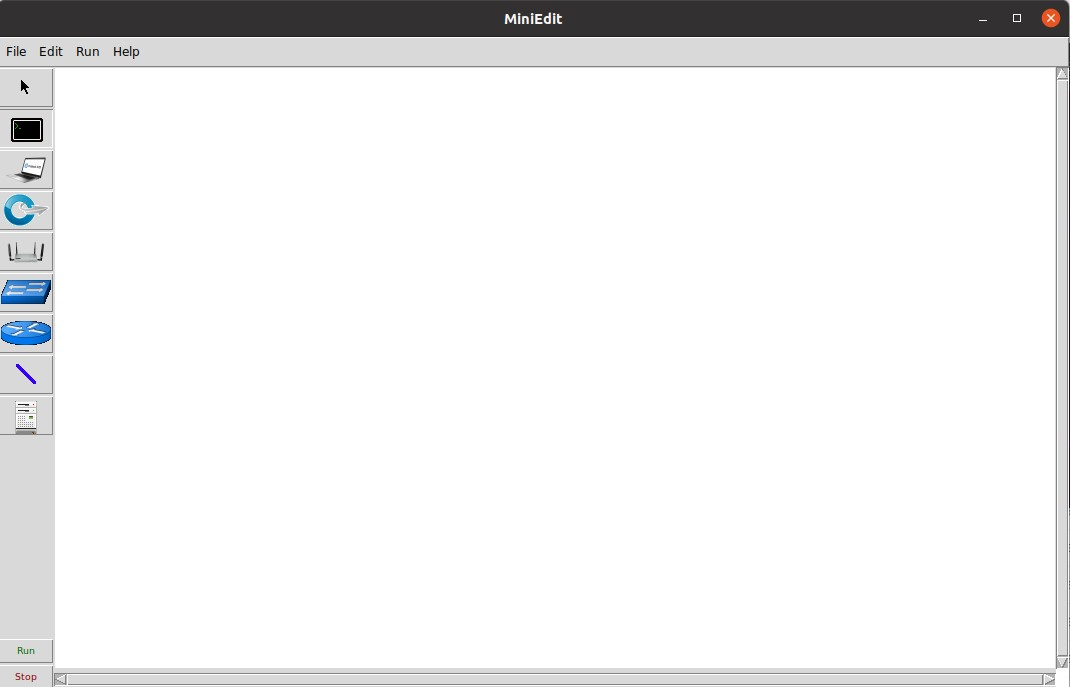
\includegraphics[width=0.85\columnwidth]{graphics/miniedit.jpg}
    \caption{Miniedit's interface for creating the network topology}
    \label{fig:miniedit}
\end{figure}

The network topology will consist of a controller, switch, host, and an access point for our WiFi network. We will then create three stations on the network, two of which will act as legitimate clients attempting to connect to the network, and the final one will be our attacker. Our access point will have two WLANs, one for clients to connect to, and one that will monitor the WiFi channels. There should be links only between the controller, switch, access point, and host.

\colorbox{lightblue}{%
\parbox{\dimexpr\linewidth-2\fboxsep}{%
\textbf{Action}

1.1.1 - Run miniedit.py, and your interface should look like Figure~\ref{fig:miniedit} above.\\
1.1.2 - Create the topology as specified above. When it is complete, it should resemble Figure~\ref{fig:miniedit_complete_topo} on page~\pageref{fig:miniedit_complete_topo} below. \\
1.1.3 - Alter the properties of the access point to have two WLANs and use channel six as seen in Figure~\ref{fig:access_point_properties} on page~\pageref{fig:access_point_properties}.
    }%
}%

Save your topology as a `.mn' file so it can be altered with Miniedit in the future if needed. Additionally, export it as a level 2 script to create a Python file you can run.

\begin{figure}[!h]
    \centering
    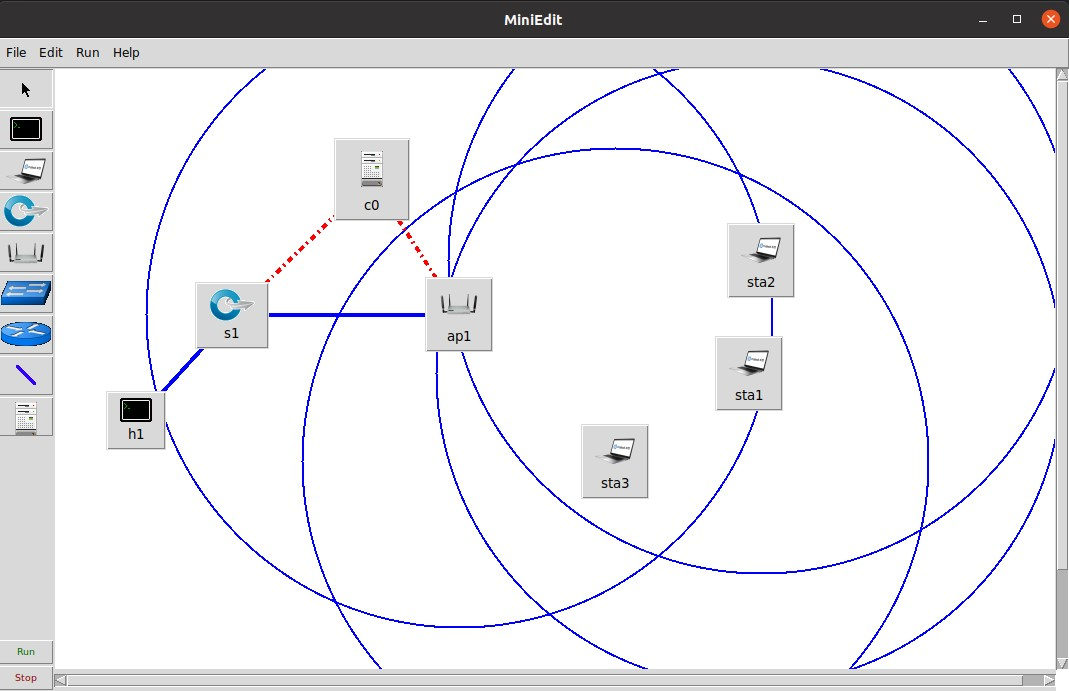
\includegraphics[width=0.8\columnwidth]{graphics/completed topology.jpg}
    \caption{Completed topology in miniedit}
    \label{fig:miniedit_complete_topo}
\end{figure}

\begin{figure}[!h]
    \centering
    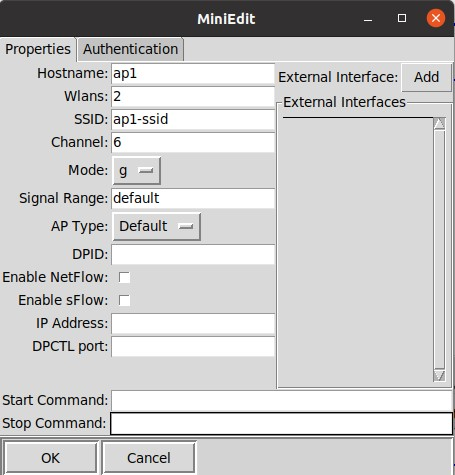
\includegraphics[width=0.65\columnwidth]{graphics/alter ap's properties.jpg}
    \caption{Right click on the access point to alter its properties}
    \label{fig:access_point_properties}
\end{figure}

\subsection*{Known Issues}\label{sec:Task-Set-1-Known-Issues}

Miniedit  will not always create an access point with two WLANs even if specified. If this is the case, manually altering the python script will be needed.

Within your exported Python script, find where the specifications of the access point are set. It should be named `ap1' and look like Figure~\ref{fig:known_issues} below. Add `wlans=2' to this line in the constructor options if it is not there.

\begin{figure}[!h]
    \centering
    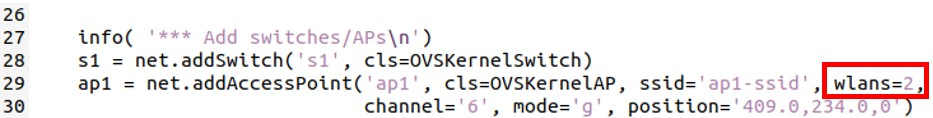
\includegraphics[width=1.2\columnwidth]{graphics/Add wlans=2.jpg}
    \caption{Add wlans=2 to your python script if it is not included by exporting from miniedit}
    \label{fig:known_issues}
\end{figure}

%%%%%%%%%%%%%%%%%%%%%%%%%%%%%%%%%%%%%%%%%
%%% Lab Task Set 2: Evil Twin Attack
%%%%%%%%%%%%%%%%%%%%%%%%%%%%%%%%%%%%%%%%%

\section*{Task Set 2: Evil Twin Attack}\label{sec:Task-Set-2}
\addcontentsline{toc}{section}{Task Set 2: Evil Twin Attack}

\textbf{Objective}

Setup an Evil Twin attack via creation of a rogue WiFi access point that appears to be legitimate but, in reality, is controlled by the attacker.

\subsection*{Task 2.1: Setting up the Evil Twin Attack}\label{sec:Task-2.1-Setting-Up-the-Evil-Twin-Attack}
\addcontentsline{toc}{subsection}{Task 2.1: Setting up the Evil Twin Attack}

The WiFi topology can now be run to set up the Evil Twin attack. The Python script exported in Task 1 will need to be run as an administrator (sudo). This will provide access to the Mininet-WiFi command-line interface. Below are some important commands that will be used within the mininet interactive terminal:

\bigskip
\begin{mdframed}
[backgroundcolor=black!10,style=code,nobreak=true,align=center,userdefinedwidth=14cm]

> nodes
\newline
Displays all nodes within the topology

> xterm <node>
\newline
Creates an external terminal to perform commands on a specific node

> py <node>.stop\_()
\newline
Stops the specified node

> py <node>.start\_()
\newline
Starts the specified node

> py <node>.setMasterMode(intf='<interface>', ssid='<desired\_ssid>', \\ channel='<desired\_channel>',  mode='g') \\
Set the node's interface to master mode allowing clients to connect to it. It allows you to specify the channel it runs on and the name of the network (ssid)

\end{mdframed}

Station 1 will be setup as the evil twin. Initially, the hardware address should be set to be the same as the LAP. By scanning for available networks, the LAP’s name and hardware address can be located. To scan for nearby networks, use the command:

\bigskip
\begin{mdframed}[backgroundcolor=black!10,style=code,nobreak=true,align=center,userdefinedwidth=14cm]
    \$ iwlist scan
\end{mdframed}

The result should look like what's shown in Figure~\ref{fig:network_scan} on page~\pageref{fig:network_scan} below.

\begin{figure}[!h]
    \centering
    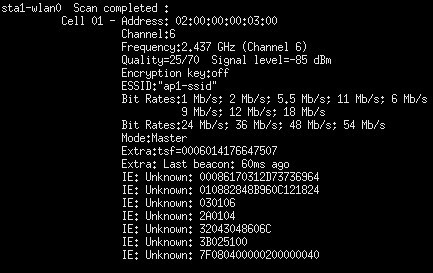
\includegraphics[width=0.9\columnwidth]{graphics/scanning_result.jpg}
    \caption{Result from scanning the network with iwlist}
    \label{fig:network_scan}
\end{figure}

The next step involves setting this interface to master mode with the LAP's Extended Service Set ID (ESSID) and evaluating the difference between placing it on the same channel versus a different one.

\colorbox{lightblue}{%
\parbox{\dimexpr\linewidth-2\fboxsep}{%
\textbf{Action}

2.1.1 - Open an xterm terminal for Station 1 and scan for available networks. \\
2.1.2 - Using the \texttt{ifconfig} cli tool, alter the hw ether on Station 1's interface to match the LAP's hardware address, and then stop and restart the node.\\
2.1.3 - Set the interface to master mode with the LAP's ESSID.\\
2.1.4 - Run the command `\texttt{\$ iw <interface> info}' to verify if the hardware address, network name, and channel are correct, and the interface is running in master mode.
    }%
}%

Finally, Station 1 will be the evil twin of the LAP. If one of the two stations is connected to the evil twin through scan, all packets should be sent to our attacker rather than the LAP.

\colorbox{lightblue}{%
\parbox{\dimexpr\linewidth-2\fboxsep}{%
\textbf{Action}

2.1.5 - Use one of the other stations to scan for networks and see what happens if the evil twin is running on the same channel vs a different channel and include the difference in your lab report.\\  
2.1.6 - Set the evil twin (Station 1) to be on the same channel as the LAP and connect station 2 to it.\\ 
2.1.7 - Verify if the client is connected to the evil twin or the LAP by running `\texttt{tcpdump}' on the access point and pinging a random IP address from the client. An easy way to tell is to also run tcpdump on the evil twin and see which one, if any, produces tcp traffic in the terminal.
    }%
}%

If the client is connected to the LAP instead of the evil twin, disconnect the client using the command below. This command will later be used by the LAP to disconnect the client from the evil twin. 
\bigskip
\begin{mdframed}
[backgroundcolor=black!10,style=code,nobreak=true,align=center,userdefinedwidth=14cm]
\$ aireplay-ng -0 0 -a <mac\_of\_access\_point> -c <\_mac\_of\_client> <monitor\_mode\_interface>
\end{mdframed}

%%%%%%%%%%%%%%%%%%%%%%%%%%%%%%%%%%%%%%%%%
%%% Task 3
%%%%%%%%%%%%%%%%%%%%%%%%%%%%%%%%%%%%%%%%%

\section*{Task Set 3: Evil Scout}\label{sec:Task 3: Evil Scout}
\addcontentsline{toc}{section}{Task Set 3: Evil Scout}

\textbf{Objective}

Learn how to implement Evil Scout.

\bigskip

Evil Scout is a defensive mechanism designed to detect and neutralize the threat posed by an Evil Twin attack. It works by capturing and analyzing the packets being sent over a network to attempt to spot any anomalies or intrusion attempts.

\subsection*{Task 3.1: Creating the Capture File}\label{sec:Task-3.1-Creating-the-Capture-File}
\addcontentsline{toc}{subsection}{Task 3.1: Creating the Capture File}

With an evil twin capturing the client’s packets on the network, it is now possible to implement Evil Scout to defend against it.

This involves capturing all packets that are sent over WiFi to the LAP’s mac address then analyzing them to detect an evil twin. The program \texttt{airodump-ng} from the aircrack-ng software suite (preinstalled on the provided VM) will be used for this purpose. This program will also be used to facilitate the disconnection of the client from the evil twin, ensuring no harm can be done by their captured packets.

If the network was set up correctly, the LAP should have two WLANs. One is used for clients to access, and the second is used to monitor network traffic. Through the below command’s interface, many specifications about the network can be seen.

\bigskip

\begin{mdframed}[backgroundcolor=black!10,style=code,nobreak=true,align=center,userdefinedwidth=14cm]
    \$ airodump-ng <monitor\_mode\_interface>
\end{mdframed}

\colorbox{lightblue}{%
\parbox{\dimexpr\linewidth-2\fboxsep}{%
\textbf{Action}

3.1.1 - Set the second WLAN on the access point to monitor mode instead of master mode.\\
3.1.2 - Run the `\texttt{airodump-ng}' command above on the LAP. Your terminal should look like Figure~\ref{fig:airodump-ng} below.\\
3.1.3 - Try sending packets from the client to the evil twin.\\
3.1.4 - Note in your lab report which field(s) increase.
    }%
}%

\begin{figure}[!h]
    \centering
    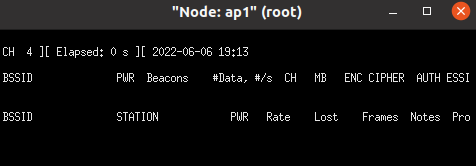
\includegraphics[width=1\columnwidth]{airodump-ng.png}
    \caption{Airodump-ng's interface}
    \label{fig:airodump-ng}
\end{figure}

Once this is complete, a capture file can be created using the command below for use with evil scout.

\bigskip

\begin{mdframed}[backgroundcolor=black!10,style=code,nobreak=true,align=center,userdefinedwidth=14cm]
    \$ airodump-ng -{}-bssid <lap\_mac\_address> -{}-channel <lap\_channel> -{}-write <filename> <monitor\_mode\_interface>
\end{mdframed}

With the above command active, send a couple pings from the client to the evil twin so the capture file has some data. Once you have a couple of packets, you can stop \texttt{airodump-ng} while focusing the termainl it's running in and using the key combo CTRL+C. You should then see a `.cap' file in the Documents directory with your specified filename.

\subsection*{Task 3.2: Implementing Evil Scout}\label{sec:Task-3.2-Implementing-Evil-Scout}
\addcontentsline{toc}{subsection}{Task 3.2: Implementing Evil Scout}

Inside the Documents directory, there is a Python script titled `EvilScout.py'. This program will implement two of the four cases that Evil Scout uses to detect the presence of evil twins.

In the first case, it checks to see if the IP prefix assigned to the client is the same prefix that is assigned to legitimate clients. In the second case, it checks the hardware source address to see if it matches any connected clients. Since only packets that intend to reach the LAP are captured, disconnecting clients connected to other LAPs poses no risk.

\colorbox{lightblue}{%
\parbox{\dimexpr\linewidth-2\fboxsep}{%
\textbf{Action}

3.2.1 - Complete EvilScout.py, using the code skeleton for the script (Figure~\ref{fig:Evil_Scout_Skeleton} on page~\pageref{fig:Evil_Scout_Skeleton}) provided in the Documents directory, and run it on the LAP. Include pictures of your completed EvilScout script and the result of running it on the LAP in your lab report.
    }%
}%

\begin{figure}[!h]
    \centering
    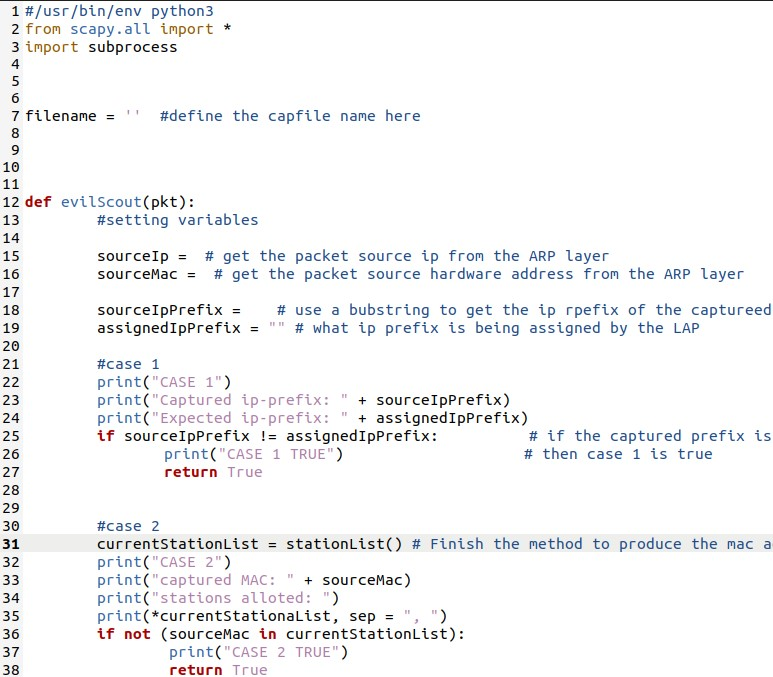
\includegraphics[width=1.2\columnwidth]{graphics/evillScout_skeleton.jpg}
    \caption{Evil Scout code skeleton to be completed}
    \label{fig:Evil_Scout_Skeleton}
\end{figure}

For case two, a list of the current stations connected to the LAP must be created. The script `station\_list\_testing.py' is included in the Documents directory to make this easier to test. It can also be seen in Figure \ref{fig:station_list_testing} below.

\begin{figure}[!h]
    \centering
    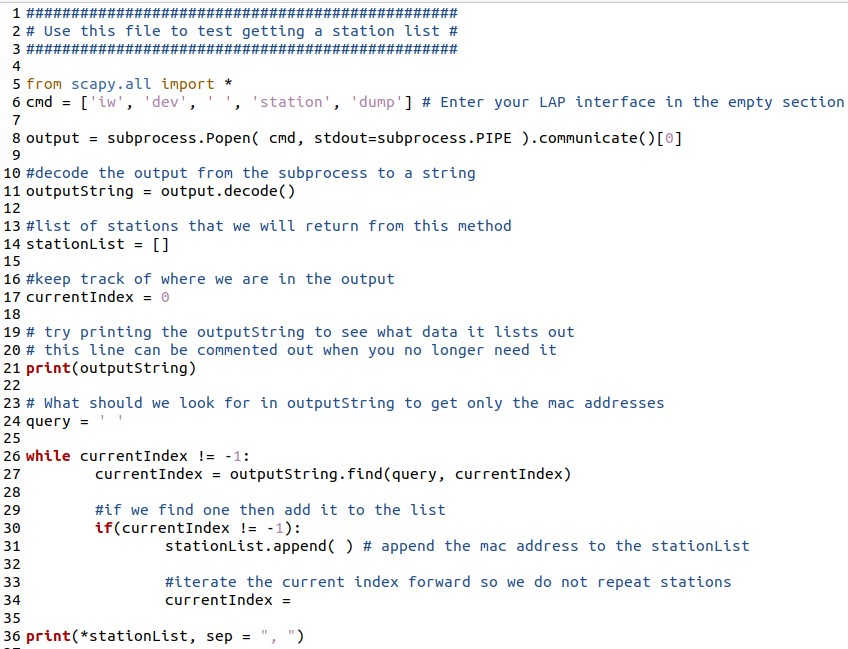
\includegraphics[width=1.2\columnwidth]{graphics/station_list_testing_ex.jpg}
    \caption{station\_list\_testing.py script to test acquisition of the LAP station list easily}
    \label{fig:station_list_testing}
\end{figure}

The completed Evil Scout script should display a message along the lines of "Evil Twin Detected!" if there's an Evil Twin and "No Evil Twin Detected!" if there isn't one. When you are satisfied with your evil scout implementation, you can move on to Task 3.3.

\subsection*{Task 3.3: Disconnecting the Client}\label{sec:Task-3.3-Disconnecting-the-Client}
\addcontentsline{toc}{subsection}{Task 3.3: Disconnecting the Client}

Aireplay-ng also allows for sending deauthentication packets to clients to make them disconnect from a network. It's essential to confirm that the client is connected to an evil twin and not the legitimate access point before sending a deauthentication. After the deauthentication, they can attempt to connect to the valid network. 

Use the command below to send this packet.

\bigskip

\begin{mdframed}[backgroundcolor=black!10,style=code,nobreak=true,align=center,userdefinedwidth=14cm]
\# aireplay-ng  -0 0 -a <mac\_of\_access\_point> -c <mac\_of\_client> <monitor\_mode\_interface>
\end{mdframed}

\bigskip

The first zero in the command is the flag used to indicate that this will be a deuathentication that is being sent. The second zero is to specify the number of packets that will be sent. Making this value 0 makes them send continuously.

\colorbox{lightblue}{%
\parbox{\dimexpr\linewidth-2\fboxsep}{%
\textbf{Action}

3.3.1 - Run \texttt{iwconfig} on the client and ensure that it is connected to the evil twin.\\
3.3.2 - Run the `\texttt{aireplay-ng}' command  above after and compare the difference.\\
3.3.3 - Include your observations in your lab report.
    }%
}%

%%%%%%%%%%%%%%%%%%%%%%%%%%%%%%%%%%%%%%%%%
%%% Task 4: Game Theory
%%%%%%%%%%%%%%%%%%%%%%%%%%%%%%%%%%%%%%%%%

\section*{Task Set 4: Adversarial Thinking for Games with Imperfect Information}\label{sec:Task 4: Game Theory}
\addcontentsline{toc}{section}{Task Set 4: Adversarial Thinking for Games with Imperfect Information}

\textbf{Objective}

Gain an understanding of adversarial thinking by being presented a hypothetical cybersecurity situation that highlights the strategic choices and trade-offs faced by both the defender and attacker.

\subsection*{Task 4.1: Adversarial Thinking}\label{Task-4.1-Adversarial-Thinking}
\addcontentsline{toc}{subsection}{Task 4.1: Adversarial Thinking}

Imagine a scenario where you setup a server that happens to be vulnerable to an attacker using an evil twin attack.

An attacker can choose to either attack the server or do nothing. If they attack, they can then choose to have the evil twin exist for a long time, defined as a long attack, or for a short amount of time, defined as a short attack.

As the server, you do not know whether the attacker is performing a long attack or a short attack, and you must decide whether to implement evil scout or do nothing. The advantage to doing nothing is that your users would be unaware that there was a data breach and your company's stock price would not decrease, but you run the risk of sensitive data being stolen. The longer the attack, the more data has the potential to be lost. The attacker also wants the server to use more resources in defending the attack, so making them implement Evil Scout from a short attack benefits the attacker as well.

Let's look at the game theory table presented in Figure~\ref{fig:subgame} below. 

\begin{figure}[h]
    \centering
    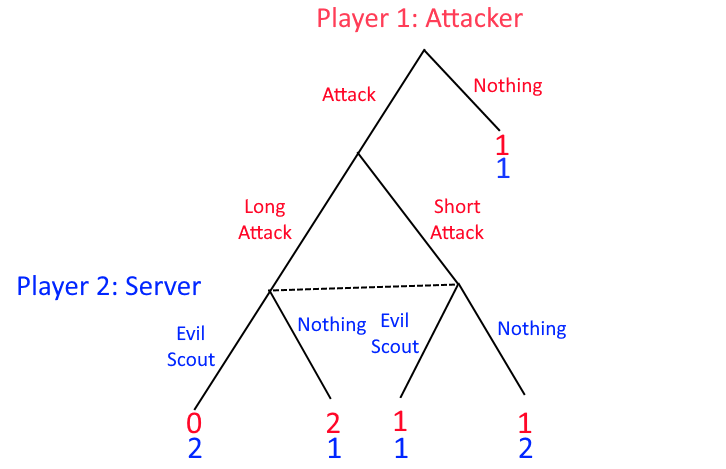
\includegraphics[width=0.9\columnwidth]{subgame.png}
    \caption{Game Theory table with imperfect information}
    \label{fig:subgame}
\end{figure}

Read, understand, and analyze the table to answer the following questions. Be sure to include the questions in your lab report. The dotted line represents that Player 2 does not know the action that Player 1 will take, which is called \textit{imperfect information}. Both players can see the table and must play based on their assumptions of what the other player will do.

\colorbox{lightblue}{%
\parbox{\dimexpr\linewidth-2\fboxsep}{%
\textbf{Action}

4.1.1 - Should player one always choose to attack? Why or why not?\\
4.1.2 - When attacking, should a short or long attack be used? Explain.\\
4.1.3 - Knowing that the server is unaware of the attack being short or long, should player 2 implement evil scout or do nothing? Explain.\\
    }%
}%

%%%%%%%%%%%%%%%%%%%%%%%%%%%%%%%%%%%%%%%%%
%%% Submission
%%%%%%%%%%%%%%%%%%%%%%%%%%%%%%%%%%%%%%%%%

\section*{Submission}\label{sec:Submission}
\addcontentsline{toc}{section}{Submission}

Submit a lab report using the provided \href{https://docs.google.com/document/d/1f_rB22EzL8aezExZ7jYFARnuy5xuhcwC/edit?usp=sharing&ouid=113481593569562690929&rtpof=true&sd=true}{lab report template}. Submit the lab report to your instructor with what you struggled with, what you learned, and images depicting the steps you took. Additionally, include your code for the evilScout.py python script. Include answers to the questions in task 4. Text and images are required for full points.

%%%%%%%%%%%%%%%%%%%%%%%%%%%%%%%%%%%%%%%%%
%%% Summary
%%%%%%%%%%%%%%%%%%%%%%%%%%%%%%%%%%%%%%%%%

\section*{Summary}\label{sec:Sumarry}
\addcontentsline{toc}{section}{Summary}

This lab explored the insecurity of public WiFi, a relatively simple way to set up an evil twin which can capture client packets, how a network can defend against this type of attack, and the implications of implementing this kind of defense from a Game Theory perspective.

The Evil Scout defense against Evil Twin attacks can be implemented in networks with just a software update and does not require any client-side work or additional hardware used in previous methods of defense. This allows for quick, easy, and efficient deployment of detection for Evil Twin attacks.

\bibliography{References}
\bibliographystyle{plain}

\end{document}

%%%%%%%%%%%%%%%%%%%%%%%%%%%%%%%%%%%%%%%%%